
%(BEGIN_QUESTION)
% Copyright 2015, Tony R. Kuphaldt, released under the Creative Commons Attribution License (v 1.0)
% This means you may do almost anything with this work of mine, so long as you give me proper credit

Suppose coil {\tt 51-2 SI} fails open in this protective relay system:

$$\includegraphics[width=15.5cm]{i02876x01.eps}$$

First, would this fault have any immediate effect on the operation of this system?  That is to say, would anyone notice the open-coil fault occurred at the precise moment it happened?

\vskip 10pt

Next, identify how the protective function of this relay would be compromised due to this coil failing open.  In other words, what abnormal power system condition(s) could go uncleared by the relay because the coil has failed?

\vskip 10pt

\underbar{file i02876}
%(END_QUESTION)





%(BEGIN_ANSWER)

There will be no immediate action as a result of the fault, because the open seal-in coil actually {\it prevents} the relay from tripping on a time-overcurrent condition.

\vskip 10pt

If the coil is failed open, there will be no time-overcurrent protection for the second phase of the power line.  This means a persistent overcurrent condition could occur and the breaker will not shut off to protect the system from damage.

%(END_ANSWER)





%(BEGIN_NOTES)

{\bf This question is intended for exams only and not worksheets!}.

%(END_NOTES)


